% Тут используется класс, установленный на сервере Papeeria. На случай, если
% текст понадобится редактировать где-то в другом месте, рядом лежит файл matmex-diploma-custom.cls
% который в момент своего создания был идентичен классу, установленному на сервере.
% Для того, чтобы им воспользоваться, замените matmex-diploma на matmex-diploma-custom
% Если вы работаете исключительно в Papeeria то мы настоятельно рекомендуем пользоваться
% классом matmex-diploma, поскольку он будет автоматически обновляться по мере внесения корректив
%
\documentclass{matmex-diploma-custom}

\usepackage{amsmath}
\usepackage{tikz}
\usetikzlibrary{bayesnet}
\pgfdeclarelayer{bg}    % declare background layer
\pgfsetlayers{bg,main}  % set the order of the layers (main is the standard layer)
\usepackage{multirow}

\begin{document}
% Год, город, название университета и факультета предопределены,
% но можно и поменять.
% Если англоязычная титульная страница не нужна, то ее можно просто удалить.
\filltitle{ru}{
    chair              = {Кафедра информационных систем},
    title              = {Разработка программного компонента для проведения сравнительного анализа биологических данный FAIRE-seq},
    % Здесь указывается тип работы. Возможные значения:
    %   coursework - Курсовая работа
    %   diploma - Диплом специалиста
    %   master - Диплом магистра
    %   bachelor - Диплом бакалавра
    type               = {bachelor},
    position           = {студента},
    group              = 4511,
    author             = {Бутомов Артем Сергеевич},
    supervisorPosition = {магистр},
    supervisor         = {Лебедев Сергей Андреевич},
    reviewerPosition   = {аспирант},
    reviewer           = {Сергушичев Алексей Александрович},
    chairHeadPosition  = {профессор, д.т.н.},
    chairHead          = {Парфенов Владимир Глебович},
    university         = {Санкт-Петербургский национальный исследовательский университет информационных технологий, механики и оптики},
    faculty            = {Факультет информационных технологий и программирования},
%   city               = {Санкт-Петербург},
%   year               = {2013}
}
%\filltitle{en}{
%    chair              = {Chair of Information Systems},
%    title              = {Development of a software component for a comparative analysis of the biological FAIRE-seq data},
%    author             = {Artiom Butomov},
%    supervisorPosition = {},
%    supervisor         = {Sergei Lebedev},
%    reviewerPosition   = {postgraduate},
%    reviewer           = {Alexey Sergushichev},
%    chairHeadPosition  = {professor, D.T.S},
%    chairHead          = {Vladimir Parfenov},
%    university         = {Saint Petersburg National Research University of Information Technologies, Mechanics and Optics},
%    faculty            = {Faculty of Information Technology and Software Engineering},
%}
\maketitle
\tableofcontents
% У введения нет номера главы
\newpage
\newpage

\section*{Введение}

ДНК (дезоксирибонуклеиновая кислота) --- длинная двухцепочечная молекула, являющаяся носителем генетической информации в биологических организмах.

В клетке ДНК упакована, то есть убирается в маленькую по размеру клетку.

Изучать пространственную структуру ДНК организма важно для понимания механизмов регуляции жизнедеятельности клетки.

Формальдегидная изоляция регуляторных элементов с последующим секвенированием (Formaldehyde-Assisted Isolation of Regulatory Elements sequencing, FAIRE-Seq) --- это биологический протокол, позволяющий находить участки, в которых ДНК доступна для связывания белками. Суть протокола заключается в том, что выделенную из клетки ДНК фиксируют на белки с помощью формальдегида. Затем ДНК фрагментируют с помощью ультразвука. После этого происходит разделение полученных фрагментов ДНК на две группы: участки связанные с белками и свободные участки. Далее свободные фрагменты читают с помощью секвенатора. И наконец, для каждого прочтения секвенатора определяют место в геноме исследуемого организма, откуда он был прочитан.

В контексте данной работы, геном разбивается на неперескающиеся отрезки фиксированной длины, называемые бинами. Подсчитывается количество прочтений, начинающихся внутри каждого отрезка. Таким образом, получатся вектор из неотрицательных целых чисел, именуемый вектором покрытия.

Из вектора покрытия можно сделать предположение о вероятности расплетения региона, чем больше значение элемента вектора, тем больше вероятность, что регион, соответствующий элементу, был расплетен.

Однако, рассматриваемый протокол не исключает возможности наличия ошибок в результатах биологического эксперемента. Неточности метода FAIRE-seq обусловлены следующими моментами.
\begin{enumerate}
\item
Протокол работает с колонией клеток. Таким образом в результатах эксперимента мы видим некоторое среднее состояние по всем клеткам
\item
Этап фиксации не обладает 100\% КПД, то есть некоторые белки могут отвалиться 
\item
Этап разделения свободных и связанных фаз также неточен. Вместе со свободными вполне могут попасться и связанные фрагменты
\end{enumerate}

Так как в результате эксперемента появляется шум, данные FAIRE-seq удобно анализировать с помощью вероятностых моделей.

Цель данной работы --- разработать математическую модель для проведения сравнительного анализа нескольких эксперементов биологический данных FAIRE-seq и научиться оценивать и контролировать число неверных предсказаний модели. 
\\\\
Для достижения цели были поставлены следующие задачи:
\begin{enumerate}
\item
Изучить предметную область
\item
Предложить несколько вероятностных моделей для сравнения экспериментов FAIRE-seq
\item
Реализовать модели в виде программы на языке Python
\item
Оценить эффективность полученной программы
\end{enumerate}

\section{Предлагаемые модели}
\subsection{Описание задачи}

Пусть $\vec{x}=(x_1,..,x_N)$ --- вектор прочтений, построенный из какого-то BAM файла.
Сопоставим каждому наблюдению некоторую метку-состояние $s_n$ из множества базовых состояний $s=\{+, --, \operatorname{null}\}$, истинные значения которых не знаем. Каждое базовое состояние описывает ситуацию в одном образце.

Вероятностная модель позволяет найти наиболее правдоподобную последовательность состояний.

\newcommand{\argmax}{\mathop{\rm arg~max}\limits}
$$\hat{s}_{ML} = \argmax_{i \in {1,..,S}^N} \mathcal{P}(x,s;\theta)$$

\subsection{Смесь многомерных распределений Пуассона}

%Будем считать, что мы работаем с двумя векторами покрытия.
%Тогда наблюдение $x_n$ - это пара чисел, каждое из которых соответствует одному %вектору $\vec{x}=\{\vec{x_1},\vec{x_2}\}$.

%Пусть $S = \{+, -\}$ — множество состояний, которые мы будем называть "базовыми%" состояниями. Каждое из базовых состояний описывает ситуацию в одном образце, %например, $(+)$ — сигнал есть, $(-)$ - шум или сигнала нет. 

%Для задачи сравнения нам нужно множество состояний, описывающее, что происходит %в каждом из образцов, то есть $S^2 = \{(+, +), (-, -), (+, -), (-, +)\}$.

Будем моделировать количество прочтений вдоль генома с помощью смеси многомерных распределений Пуассона. Пусть $\pi = (\pi_1,..,\pi_S)$ --- априорные вероятности компонент. Причем, $\sum_{}\pi_i = 1$

$\lambda = (\lambda_1,..,\lambda_S)$ --- параметры пуассоновских испусканий для каждой компоненты смеси. Тогда правдоподобие неполных данных записывается так:

\begin{equation}
p(x;\pi,\lambda) = \prod_{n=1}^N\sum_{i=1}^S\pi_i\mathcal{P}(x_n;\lambda_i)
\end{equation}

Интерпретация в качестве порождающей модели следующая\cite{book:flach}: сначала случайным образом выбираем скрытое состояние, применяя распределение $\pi$, а затем используем выбранное скрытое состояние для порождения наблюдения.

\begin{figure}[h!]
  \centering
  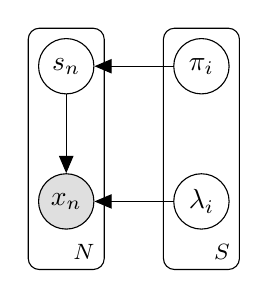
\begin{tikzpicture}
    \node[latent]              (pi) {$\pi_i$};
    \node[latent, left=of pi] (z)  {$s_n$};
    \node[latent, below=of pi] (l)  {$\lambda_i$};
    \node[obs, below=of z]     (x)  {$x_n$};

    \edge {pi} {z};
    \edge {l,z} {x};

    \plate {pip} {(pi)(l)} {$S$};
    \plate {xlz} {(x)(z)} {$N$};
  \end{tikzpicture}
  \caption{Графическая диаграмма для пуассоновской смеси}
  \label{fig:generative-mm}
\end{figure}

Чтобы найти параметры модели с помощью оценки максимального правдоподобия, следует обратить в максимум совместное правдоподобие наблюдаемых и скрытых переменных. Методом максимального правдоподобия найти решение довольно сложно, поскольку для этого требуется решить систему, где оцениваемые параметры зависят от наблюдаемой выборки $x$ и неизвестных значений скрытых состояний $s$. Асимптотическая сложность решения возрастет в $S^N$ раз.

Поэтому будем искать приближенное решение с помощью EM-алгоритма, в котором нижняя оценка правдоподобия оптимизируется до сходимости. Последовательность действий формируется следующим образом\cite{book:Bishop}:
\begin{enumerate}
\item
Инициализировать начальные значения параметров
\item
Присвоение ожидаемых значений скрытым переменным при условии текущих оценок параметров и нахождение математического ожидания правдоподобия.
$$\mathrm{Q}(\theta|\theta^{\operatorname{old}})
=\mathrm{E}[\log p(x,s;\theta)]\le \log p(x;\theta)$$
\item
Переоценка параметров с учетом обновленных ожидаемых значений скрытых переменных
$$\theta^{\operatorname{new}}=\argmax_{\theta \in \Theta} \mathrm{Q}(\theta|\theta^{\operatorname{old}})$$
\item
Вычислить логарифм правдоподобия и проверить на сходимость
\end{enumerate}

Выведем EM-алгоритм для смеси многомерных Пуассоновских испусканий.

Запишем логарифм функции правдоподобия:

\begin{equation}
\ln p(x;\pi,\lambda) = \sum_{n=1}^N \ln{\sum_{i=1}^S} \pi_i \mathcal{P}(x_n;\lambda_i)
\end{equation}

\subsection*{Шаг E}

\begin{equation}
\gamma(s_{ni}) = \frac{\pi_i\mathcal{P}(x_n;\lambda_i)}{\sum_{j=1}^S\pi_j\mathcal{P}(x_n;\lambda_j)}
\end{equation}

\subsection*{Шаг М}

Чтобы максимизировать логарифмическое правдоподобие относительно параметров, необходимо взять частные производные и приравнять их к нулю.

% вместо |  - использовать ;
\begin{align*}
\frac{\partial}{\partial \lambda_i}\mathrm{E}[\log p(x;s,\theta)]\\
&=\frac{\partial}{\partial \lambda_i}\sum_{n=1}^N \sum_{s=1}^S
\mathrm{E}[s_{ni}]\{\log \pi_i + \log \mathcal{P}(x_n|\theta)\}\\
&= \sum_{n=1}^N \mathrm{E}[s_{ni}] \frac{\partial}{\partial \lambda_i} \log \mathcal{P}(x_n|\theta)\\
&= \sum_{n=1}^N \gamma(s_{nk}) \frac{\partial}{\partial \lambda_i} \log {\frac{\lambda^{x_n} e^{-\lambda}}{x_n!}}\\
&= \sum_{n=1}^N \gamma(s_{nk}) \frac{\partial}{\partial \lambda_i} (\log {\lambda_i}^{x_n} + \log e^{-\lambda_k} - \log x_n! )\\
&= \sum_{n=1}^N \gamma(s_{ni}) \frac{\partial}{\partial \lambda_i} (x_n \log \lambda_i - \lambda_i - \log x_n! )\\
&= \sum_{n=1}^N \gamma(s_{ni}) (\frac{x_n}{\lambda_S} - 1)\\
&= 0
\end{align*}
%$$\frac{\partial}{\partial \lambda_i}\mathrm{E}[\log p(x;s,\theta)]$$
%$$=\frac{\partial}{\partial \lambda_i}\sum_{n=1}^N \sum_{s=1}^S
%\mathrm{E}[s_{ni}]\{\log \pi_i + \log \mathcal{P}(x_n|\theta)\}$$
%$$= \sum_{n=1}^N \mathrm{E}[s_{ni}] \frac{\partial}{\partial \lambda_i} \log %\mathcal{P}(x_n|\theta)$$
%$$= \sum_{n=1}^N \gamma(s_{nk}) \frac{\partial}{\partial \lambda_i} \log %{\frac{\lambda^{x_n} e^{-\lambda}}{x_n!}}$$
%$$= \sum_{n=1}^N \gamma(s_{nk}) \frac{\partial}{\partial \lambda_i} (\log %{\lambda_i}^{x_n} + \log e^{-\lambda_k} - \log x_n! )$$
%$$= \sum_{n=1}^N \gamma(s_{ni}) \frac{\partial}{\partial \lambda_i} (x_n \log %\lambda_i - \lambda_i - \log x_n! )$$
%$$= \sum_{n=1}^N \gamma(s_{ni}) (\frac{x_n}{\lambda_S} - 1)= 0$$
\\\\
получаем
\begin{equation}
\lambda_i^* = \frac{1}{N_i}\sum_{n=1}^N\gamma(s_{ni})x_n
\end{equation}
\\\\
где
\begin{equation}
N_i = \sum_{n=1}^N\gamma(s_ni)
\end{equation}
Найдем новые значения априорных вероятностей.
Воспользуемся методом множителей Лагранжа для учета ограничений на вектор априорных вероятностей.

\begin{align*}
\frac{\partial}{\partial \pi_i}( \mathrm{E}[\log p(x;s,\theta)] &+ \lambda(\sum_{j=1}^S \pi_j - 1))
\\&= \frac{\partial}{\partial \pi_i}\sum_{n=1}^N \sum_{i=1}^S
E[s_{ni}]\{\log \pi_i + \log \mathcal{P}(x_n;\theta)\} + \frac{\partial}{\partial \pi_i}\lambda(\sum_{j=1}^S \pi_j - 1)
\\& = \sum_{n=1}^N
\gamma(s_{ni})\frac{\partial}{\partial \pi_i}\{\log \pi_i + \log \mathcal{P}(x_n|\theta)\} + \frac{\partial}{\partial \pi_i} \lambda(\sum_{j=1}^S \pi_j - 1)\\
&=\sum_{n=1}^N
\gamma(s_{ni})\frac{\partial}{\partial \pi_i}\{\log \pi_i\} + \frac{\partial}{\partial \pi_i} \lambda(\sum_{j=1}^S \pi_j - 1) \\
&=\sum_{n=1}^N
\gamma(s_{ni})\frac{1}{\pi_i} + \lambda \\&= 0
\end{align*}
%$$\frac{\partial}{\partial \pi_i}( \mathrm{E}[\log p(x;s,\theta)] + \lambd
%(\sum_{j=1}^S \pi_j - 1))$$
%$$= \frac{\partial}{\partial \pi_i}\sum_{n=1}^N \sum_{i=1}^S
%E[s_{ni}]\{\log \pi_i + \log \mathcal{P}(x_n;\theta)\} + \frac{\partial}{\parti%al \pi_i}\lambda(\sum_{j=1}^S \pi_j - 1)$$
%$$ = \sum_{n=1}^N
%\gamma(s_{ni})\frac{\partial}{\partial \pi_i}\{\log \pi_i + \log \mathcal{P}%(x_n|\theta)\} + \frac{\partial}{\partial \pi_i} \lambda(\sum_{j=1}^S \pi_j - 1%)$$
%$$=\sum_{n=1}^N
%\gamma(s_{ni})\frac{\partial}{\partial \pi_i}\{\log \pi_i\} + \frac{\partial}{\%partial \pi_i} \lambda(\sum_{j=1}^S \pi_j - 1) $$
%$$=\sum_{n=1}^N
%\gamma(s_{ni})\frac{1}{\pi_i} + \lambda = 0$$
\\
Домножив на $\pi_k$, получаем
\begin{equation}
\sum_{n=1}^N \gamma(s_{ni}) + \pi_i \lambda = 0
\end{equation}
Просуммируем вдоль $i$
\begin{equation}
\sum_{n=1}^N \sum_{i=1}^S \gamma(s_{ni}) + \sum_{i=1}^S \pi_i \lambda = 0
\end{equation}
Применяя
$$\sum_{i=1}^S \gamma(s_{ni}) = 1$$
и
$$\sum_{i=1}^S \pi_i = 1$$
Из выражения (7) получаем
$$N + \lambda = 0$$
$$\lambda = -N$$
Далее, подставляя найденное $\lambda$ в выражение (6), получаем
$$\pi_i = - \frac{\sum_{n=1}^N\gamma(s_{ni})}{\lambda} = \frac{N_i}{N}$$
Наконец,
\begin{align}
\pi_{i}^* = \frac{N_i}{N} 
\end{align}

\textbf{Примечание.} Чтобы обучить наши данные, следует проинициализировать начальные значения входных параметров модели. Для этой задачи можно использовать алгоритм кластеризации KMeans++\cite{book:murphy}, который разбивает наши наблюдения на $S$ кластеров. Работа алгоритма основана на методе максимального правдоподобия. На шаге Е мы определяем для каждого наблюдения ближайший кластер. На шаге М Вычисляем новое значение кластера, которое принимаем за среднее выборочное наблюдений, относящихся к данному кластеру. Алгоритм итерируется до тех пор, пока изменения логарифма правдоподобия не станет меньше константы. В результате, начальные значений параметров Пуассоновского распределения можно принять за значения кластеров.
% TODO Смотри замечания научрука.

\newpage
\subsection{Скрытая Марковская Модель}

На практике предположение о независимости  состояний между соседними наблюдениями в предыдущей модели не выполняется.

Поэтому, перейдем к Скрытой Марковской Модели второго порядка, чтобы учесть зависимость между состояниями соседних наблюдений.

\begin{figure}[h!]
  \centering
  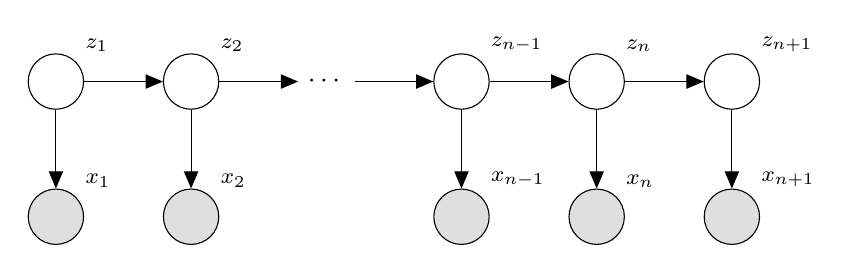
\begin{tikzpicture}]
  
    \node[latent, label=above right:$z_1$] (z1) {};
    \node[latent, right=of z1, label=above right:$z_2$] (z2) {};
    \node[draw=none, right=of z2] (ellipsis) {$\cdots$};
    \node[latent, right=of ellipsis, label=above right:$z_{n-1}$] (zn) {};
    \node[latent, right=of zn, label=above right:$z_{n}$] (znn) {};
    \node[latent, right=of znn, label=above right:$z_{n+1}$] (znnn) {};
    
    \edge {z1} {z2};
    \edge {z2} {ellipsis};
    \edge {ellipsis} {zn};
    \edge {zn} {znn};
    \edge {znn} {znnn};
    \edge {znnn} {};
    
    \node[obs, below=of z1, label=above right:$x_1$] (x1) {};
    \node[obs, below=of z2, label=above right:$x_2$] (x2) {};

    \node[obs, below=of zn, label=above right:$x_{n-1}$] (xn) {};
    \node[obs, below=of znn, label=above right:$x_{n}$] (xnn) {};
    \node[obs, below=of znnn, label=above right:$x_{n+1}$] (xnnn) {};
    
    \edge {z1} {x1};
    \edge {z2} {x2};
    \edge {zn} {xn};
    \edge {znn} {xnn};
    \edge {znnn} {xnnn};

  \end{tikzpicture}
  \caption{Графическая диаграмма для марковской цепи}
  \label{fig:generative-mm}
\end{figure}

\[
z_{(n+1),i} \mbox{ зависит от } z_{n,i}
\]

Введем понятие базовых состояний: $ S \in \{+, -, \operatorname{null}\}$.
Каждое из базовых состояний описывает ситуацию в одном образце. 

Семантика обозначений следующая:
\\
$(+)$ - сигнал есть,  $(-)$ - шумовый сигнал, $\operatorname{(null)}$ - сигнала нет.
\\\\
\textbf{Замечание.} Отличие $\operatorname{(null)}$ от $(-)$ заключаются в полном отсутствии сигнала.
\\\\
Для задачи сравнения нам нужно множество состояний, описывающее, что происходит в каждом из образцов, то есть $S^2$.
\\\\
Состояние $s$ с одинаковым базовыми состояниями $(+,+),(-,-),(\operatorname{null},\operatorname{null})$ означает, что данные сравниваемых образцов наблюдения $x_n$ похожи между собой.
\\\\

Чтобы задать модель, нужно определить распределения испусканий, то есть $p(x_n;s_{ni} = 1)$, где i — индекс состояния из $S^2$, а n — индекс наблюдения. Будем считать, что $x_n$ — это наблюдение из многомерного распределения Пуассона с независимыми компонентами, то есть:

\begin{equation}
p(x_n;s_{ni}) = \prod\limits_{d = 1}^2 p(x_{nd};\lambda_{id})
\end{equation}

На данном этапе для каждого состояния и каждого образца есть свой параметр распределения Пуассона, что является неверной параметизацией. Рассмотрим два состояния $i = (+, +)$ и $j = (+, -)$ и выпишем для них функцию вероятности распределения Пуассона:

\begin{align*}
p(x_n|s_{ni}) = \prod\limits_{d = 1}^2 p(x_{nd}|\lambda_{id}) = p(x_{n1}|\lambda_{i1}) p(x_{n2}|\lambda_{i2})
\end{align*}
\begin{align*}
p(x_n|s_{nj}) = \prod\limits_{d = 1}^2 p(x_{nd}|\lambda_{jd}) = p(x_{n1}|\lambda_{j1}) p(x_{n2}|\lambda_{j2})
\end{align*}

Первый множитель в обоих выражениях соответствует наблюдению, порождённому базовым состоянием $(+)$ в первом образце. Логично положить, что $\lambda_{i1} = \lambda_{j1}$, потому что в обратном случае испусканиям для одного и того же базового состояния будут соответствовать разные параметры распределения Пуассона. Таким образом, различных параметров у нас не $2 * |S^2| = 8$, а $2 * |S| = 4$.

Для реализации удобно представлять параметры многомерного распределения Пуассона в виде вектора размерности $2 * |S|$, а для состояния i из $S^2$ использовать матрицу трансляции D. Матрица трансляции --- это двухмерная матрица размерности $2 \times |S^2|$, где $D_{di}$ - индекс параметра из вектора:

$$\vec{\lambda}=\{\lambda_1, \lambda_2, \lambda_3, \lambda_4\, \lambda_5, \lambda_6\}$$

%\begin{figure}[h]
%\label{разрыв_функции}
%\centering
%\includegraphics[scale=0.8]{transmat.png}
%\caption{Матрица трансляции}
%\end{figure}
\begin{tabular}{cc|c|c|c|c|c|c|c|c|c|c|l}
\cline{3-11} & & (n,n) & (+,+) & (--,--) & (n,+) & (n, --) & (--, n) & (+,n) & (+, --) & (--, +) \\
\cline{1-11} \multicolumn{1}{ |c  }{\multirow{2}{*}{D} } & \multicolumn{1}{ |c| }{\multirow{1}{*}{d=1}} & 3 & 4 & 5 & 6 & 7 & 8 & 9 & 10 & 11 \\
\cline{2-11} \multicolumn{1}{ |c  }{} & \multicolumn{1}{ |c| }{d=2} & 3 & 4 & 5 & 6 & 7 & 8 & 9 & 10 & 11 \\
\cline{1-11}
\end{tabular}
\\\\
\\
Пусть

$\pi = (\pi_1,..,\pi_{S^2})$ --- априорные вероятности состояний.
    
$\mathcal{A}$ --- матрица вероятностей перехода между состояниями.

Перепишем функцию вероятности распределения Пуассона в терминах D.

\begin{equation}p(x_n;s_{ni}) = \prod\limits_{d = 1}^2 \prod\limits_{s = 1}^{|S^2|} p(x_{nd};\lambda_s)^{I[D_{di} = s]}\end{equation}

Функция правдоподобия определяется как

\begin{equation}p(x,s;\theta) = p(s_1;\pi)\bigg[\prod_{n=2}^N p(s_n;s_{n-1},A)\bigg]\prod_{m=1}^N p(x_n;s_m,\theta)\end{equation}

Подставив определение функции вероятности распределения (10) в функцию правдоподобия для СММ (11) можно убедиться, что М-шаг для вектора лямбд:

\begin{equation}\lambda_s = \frac{\sum\limits_{d = 1}^2 \sum\limits_{i = 1}^{|S^2|} I[D_{di} = s] \sum\limits_{n = 1}^N \gamma_{ni} x_{nd}}
                 {\sum\limits_{d = 1}^2 \sum\limits_{i = 1}^{|S^2|} I[D_{di} = s] \sum\limits_{n = 1}^N \gamma_{ni}}\end{equation}

\newpage
\begin{figure}[h!]
  \centering
  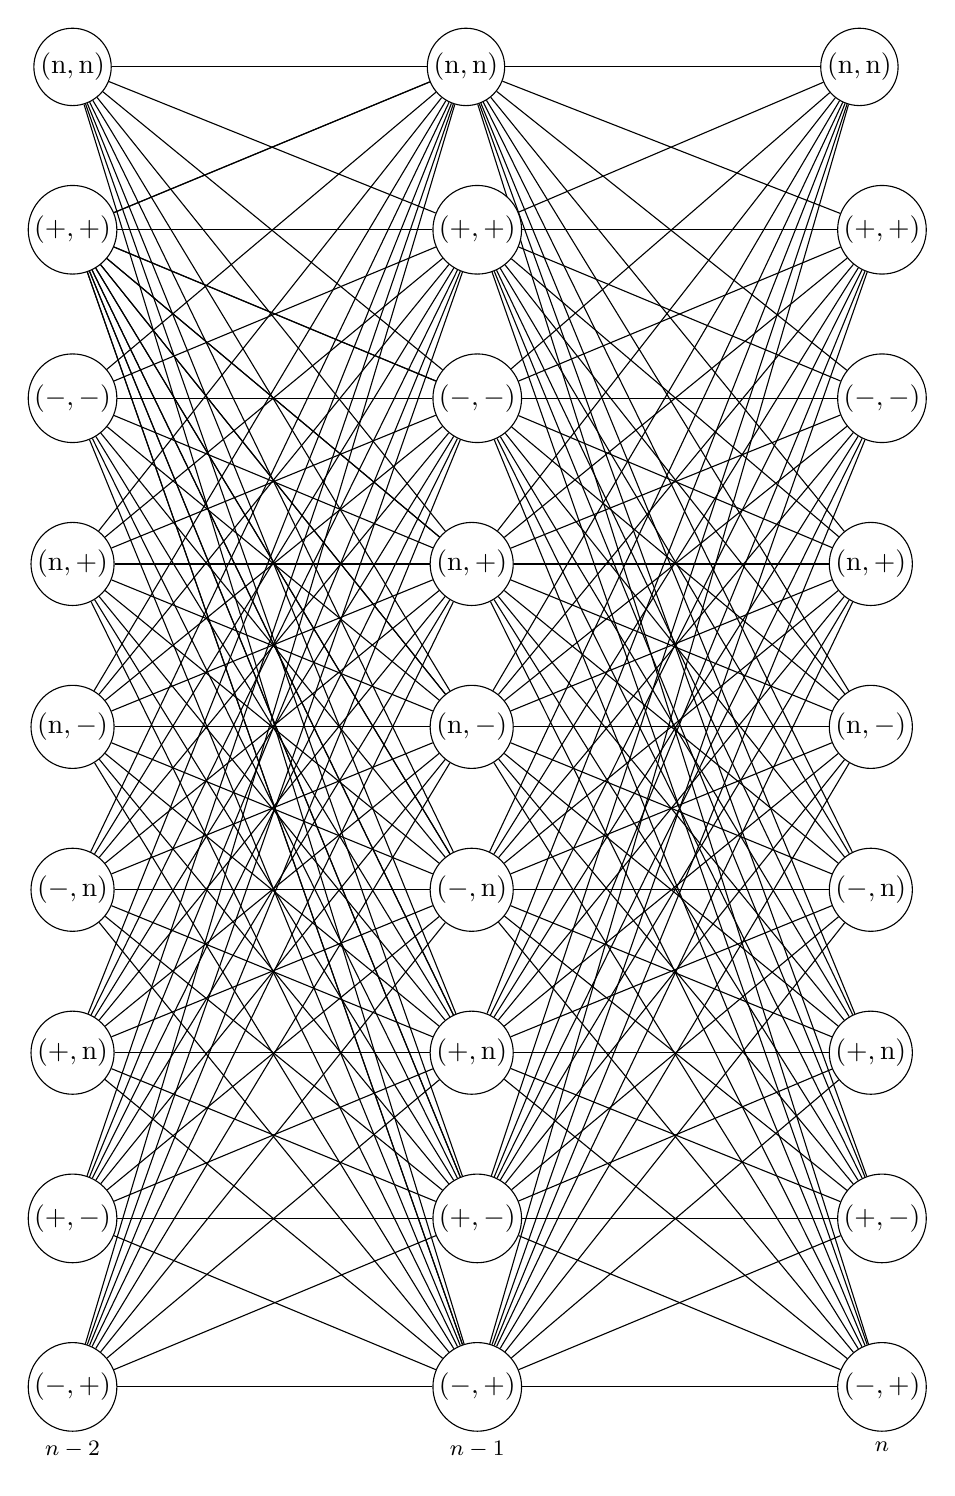
\begin{tikzpicture}[node distance=3cm and 1cm]

    \node[latent]              (s1)  {$(\operatorname{n},\operatorname{n})$};
    \node[latent, below=of s1] (s2)  {$(+,+)$};
    \node[latent, below=of s2] (s3)  {$(-,-)$};
    \node[latent, below=of s3] (s4)  {$(\operatorname{n},+)$};
    \node[latent, below=of s4] (s5)  {$(\operatorname{n},-)$};
    \node[latent, below=of s5] (s6)  {$(-,\operatorname{n})$};
    \node[latent, below=of s6] (s7)  {$(+,\operatorname{n})$};
    \node[latent, below=of s7] (s8)  {$(+,-)$};
    \node[latent, below=of s8,  label=below:$n-2$] (s9)  {$(-,+)$};
    
    \node[latent, right=of s1, xshift=3cm]     (ss1)  {$(\operatorname{n},\operatorname{n})$};
    \node[latent, right=of s2, xshift=3cm]     (ss2)  {$(+,+)$};
    \node[latent, right=of s3, xshift=3cm]     (ss3)  {$(-,-)$};
    \node[latent, right=of s4, xshift=3cm]     (ss4)  {$(\operatorname{n},+)$};
    \node[latent, right=of s5, xshift=3cm]     (ss5)  {$(\operatorname{n},-)$};
    \node[latent, right=of s6, xshift=3cm]     (ss6)  {$(-,\operatorname{n})$};
    \node[latent, right=of s7, xshift=3cm]     (ss7)  {$(+,\operatorname{n})$};
    \node[latent, right=of s8, xshift=3cm]     (ss8)  {$(+,-)$};
    \node[latent, right=of s9, xshift=3cm,  label=below:$n-1$]     (ss9)  {$(-,+)$};;
    
    \node[latent, right=of ss1, xshift=3cm]     (sss1)  {$(\operatorname{n},\operatorname{n})$};
    \node[latent, right=of ss2, xshift=3cm]     (sss2)  {$(+,+)$};
    \node[latent, right=of ss3, xshift=3cm]     (sss3)  {$(-,-)$};
    \node[latent, right=of ss4, xshift=3cm]     (sss4)  {$(\operatorname{n},+)$};
    \node[latent, right=of ss5, xshift=3cm]     (sss5)  {$(\operatorname{n},-)$};
    \node[latent, right=of ss6, xshift=3cm]     (sss6)  {$(-,\operatorname{n})$};
    \node[latent, right=of ss7, xshift=3cm]     (sss7)  {$(+,\operatorname{n})$};
    \node[latent, right=of ss8, xshift=3cm]     (sss8)  {$(+,-)$};
    \node[latent, right=of ss9, xshift=3cm, label=below:$n$]     (sss9)  {$(-,+)$};
    
    \begin{pgfonlayer}{bg}
        \edge[-] {s1,s2,s2,s3,s4,s5,s6,s7,s8,s9} {ss1,ss2,ss3,ss4,ss5,ss6,ss7,ss8,ss9};
        \edge[-] {ss1,ss2,ss3,ss4,ss5,ss6,ss7,ss8,ss9} {sss1,sss2,sss3,sss4,sss5,sss6,sss7,sss8,sss9};
    \end{pgfonlayer}

  \end{tikzpicture}
  \caption{Решетка перехода состояний}
  \label{fig:generative-mm}
\end{figure}
% Рисунок, размещенный с предпочтением "вверху страницы"
%\begin{figure}[h]
%\label{разрыв_функции}
%\centering
%\includegraphics[scale=0.9]{plate_states3.png}
%\caption{решетка состояний}
%\end{figure}
Решетка представляет собой диаграмму переходов между скрытыми состояниями модели. Красным светом выделены состояния, в котором базовые состояния похожи, то есть $(+,+),(-,-),(\operatorname{null},\operatorname{null})$

\subsection*{Шаг E}
\begin{equation}\gamma_{ni}=\frac{\alpha_{ni}\beta_{ni}}{\sum_{j=1}^{S^2}\alpha_{nj}\beta_{nj}}\end{equation}

\begin{equation}\xi_{nij}=\frac{\alpha_{(n-1),i}\mathcal{A}_{ij}\mathcal{P}(x_n;\lambda_j)\beta_{nj}}{\sum_{i'=1}^{S^2}\sum_{j'=1}^{S^2}\alpha_{(n-1),i'}A_{i'j'}\mathcal{P}(x_n;\lambda_{j'})\beta_{nj'}}\end{equation}
\\\\
Где, 
\\\\
$\alpha_{ni}=p(s_{ni}=1,x_1,x_2,..x_n;\theta)$
\\\\
$\beta_{ni}=p(x_{n+1}, ..,x_N; s_{ni}=1,\theta)$
\\\\
Вычисления $\alpha$ и $\beta$ производится с помощью алгоритма прямого-обратного хода\cite{article:rabiner}:

$$\alpha_{1i}=\pi_i\mathcal{P}$$

$$\beta_{Ni}=1$$

$$\alpha_{ni}=\mathcal{P}(x_n;\lambda_i)\sum_{j=1}^S\alpha_{(n-1),j}A_{ji}$$

$$\beta_{ni}=\sum_{j=1}^S A_{ij}\mathcal{P}(x_{n+1};\lambda_j)\beta_{(n+1),j}$$

\subsection*{Шаг М}
Новые значения параметров модели вычисляются так:
\begin{equation}\pi_i^*=\gamma(s_{1i})\end{equation}

\begin{equation}A_{ij}^*=\frac{\sum_{n=2}^N\xi_{nij}}{\sum_{j'=1}^S\sum_{n=2}^N\xi_{nij}\xi_{nij'}}\end{equation}

%\begin{equation}\lambda_i^* = \frac{\sum_{n=1}^N\gamma(s_{ni})x_n}{\sum_{n=1}^N\gamma(s_{ni})}\end{equation}

\textbf{Замечание.} В алгоритме прямого-обратного хода может быть underflow - это значит, что не хватает точности чисел с плавающей точкой.
Поэтому удобно проводить вычисления в логарифмах\cite{wiki:logsumexp}.

\subsubsection{Предсказание модели}
%Для нахождения наиболее правдоподобной последовательности скрытых состояний достаточно выбрать состояния с наибольшей апостериорной вероятностью для каждого наблюдения:
В результате работы алгоритма, необходимо предсказать наиболее вероятную последовательность скрытых состояний, породивших наши наблюдения.
Для каждого наблюдения выбирается состояние, соответствующее наибольшей апостериорной вероятности\cite{wiki:voron}.

$$s_n = \argmax_{i \in {1,..,S}^N} {\gamma (s_{ni})} $$

\subsection{Выбор модели}
Для задачи сравнения двух образцов была выбрана Скрытая Марковская Модель.
В частном случае, для анализа одного биологического образца СММ более правдоподобнее, чем смесь Пуассоновских испусканий.
%% запихнуть табличку двухстолбчатую со значениями правдоподобий некоторых хромосом: первый ст. - Смесь, второй - СММ.
Это значит, что модель, в которой предполагается зависимость между состояниями соседних наблюдений, более правдоподобная.

\subsection{Актуальности разработки}

Существуют инструменты для анализа одного эксперимента с использованием FAIRE-seq:

\begin{itemize}
  \item ChromHMM
  \item ZINBA
  \item Fseq
  \item ChIPOTle Peak Finder 
  \item и другие \ldots
\end{itemize}

\textbf{Примечание.} Косвенный аналог ChromHMM моделирует многомерную последовательность из $\{0, 1\}$. Данный инструмент, как и другие аналоги, используется для анализа одного биологического образца. Стало быть, для задачи сравнения он не подходит. Также ChromHMM не умеет моделировать репликаты(образцы).

\section{Оценка модели}

\subsection{Оценка качества работы модели}

При оценке качества работы модели мы хотели бы получать число неверных предсказаний FDR\cite{wiki:fdr} среди всех предсказаний модели. Для того чтобы ввести FDR, сформулируем гипотезы, которые будем проверять с помощью модели: 

\begin{itemize}
  \item $H_0$ - разницы между состояниями эксперементальных данных в одном наблюдении нет
  \item $H_1$ - разница есть
\end{itemize}

Рассмотрим некоторое наблюдение с индексом n в нашей выборке, cформируем критерий

\begin{itemize}
  \item $P(\textrm{отличий в n нет}; x, \theta) := p_0$
  \item $P(\textrm{отличия в n есть};x, \theta) := p_1$
\end{itemize}

$H_0$ отвергается если $p_0 < p_1$ и не отвергается в обратном случае. 

\textbf{Примечание.} Вспомним, что $p_0 + p_1 = 1$, поэтому наш критерий можно записать как:
$$p_0 \le 0.5$$

Таким образом, применив сформулированный выше критерий ко всем бинам $n = 1,..., N$ мы получим N результатов. FDR = $a \in [0, 1]$ означает, что среди N результатов $\operatorname{a}\operatorname{N}$ — неверны.

В общем виде FDR записывается так:

$\operatorname{FDR} = \operatorname{E}[\operatorname{FP} / (\operatorname{TP} + \operatorname{FP})]$,

где FP — количество неверно отвергнутых нулевых гипотез, TP — количество верно отвергнутых нулевых гипотез.

Для удобства будем использовать следующую разновидность FDR:

\begin{equation}\operatorname{mFDR} = \operatorname{E}[\operatorname{FP}] / \operatorname{E}[\operatorname{TP} + \operatorname{FP}]\end{equation}

Числитель можно представить ввиду суммы индикаторных случайных величин $\operatorname{FP}_n$

$$\operatorname{E[FP]} = \sum\limits_{n = 1}^N \operatorname{E}[\operatorname{FP}_n]$$

Если n-й учаток не содержит отличий, то $\operatorname{FP}_n = 0$. Если n-й участок по мнению модели содержит отличия, то $\operatorname{FP}_n = 1$ в случае, когда отличия действительно есть и 0 в обратном случае.

Разумеется, правильного ответа для каждого n мы не знаем, но у нас есть вероятность ошибки, а именно $P(\textrm{отличий в n нет}; x, \theta)$, которую мы обозначили за $p_1$. Посчитаем математическое ожидание:

$$\operatorname{E[FP]} = \sum\limits_{n = 1}^N I[p_1 \le 0.5] p_1$$

Здесь мы воспользовались тем, что математическое ожидание индикаторной случайной величины с параметром p равняется p.

Перейдём к знаменателю. Выражение для E[FP] у нас уже есть, построим аналогичное выражение для $\operatorname{E[TP]}$.  $\operatorname{TP}_n = 1$ если отличия в n-м участке есть, и модель с этим солидарна, и 0 — во всех остальных случаях. Заметим, что $\operatorname{TP}_n$ независимы потому же почему и $\operatorname{FP}_n$.

$$\operatorname{E[TP]}= \sum\limits_{n = 1}^N I[p_1 <= 0.5] p_0$$

Выпишем то, что получилось:

$$\operatorname{E[TP + FP]} = \sum\limits_{n = 1}^N (I[p_1 \le 0.5] p_1 + I[p_1 \le 0.5] p_0) = \sum\limits_{n = 1}^N I[p_1 \le 0.5]$$

Здесь мы воспользовались тем, что $p_0 + p_1 = 1$

И всё вместе:

$$\widehat{\operatorname{mFDR}} = \frac{ \sum\limits_{n = 1}^N I[p_1 \le 0.5] p_1}{\sum\limits_{n = 1}^N I[p_1 \le 0.5]}$$

Таким образом, оценив апостериорные вероятности мы можем также оценить и mFDR. Важно понимать, что по выборке (точнее по апостериорным вероятностям для выборки) мы получили оценку mFDR, а не его истинное значение. 

\subsection{Контроль FDR}

Мы хотим выдавать вектор предсказаний, в котором гарантированно не более чем фиксированное число ошибок.

\section{Проектирование}

С точки зрения быстроты, удобно все действия над исходными данными производить в одной инстанции, т.е в одном классе.

\begin{figure}[h]
\centering
\includegraphics[scale=0.8]{system_architecture.png}
\caption{системная архитектура}
\label{fig:system_architecture}
\end{figure}

Условное разделение программы на три компоненты. Классы Reader и Writer выделены в отдельные классы для того, чтобы показать их независимость от класса MultiPoissonHMM, т.е абстрагируемся от деталей реализации этих классов, так как каждый класс выполняет независимую и отдельную задачу. Поэтому функции ввода и вывода мы обернули в класс (см. Рис. \ref{fig:classes_diagram}). 
\\\\
Здесь будет описание диаграммы классов. Предварительно поправив саму диаграмму ...
\\\\
Здесь будет описание диаграммы последовательности...
\\\\
Программа собрана в виде проекта и состоит из файлов: 
$\operatorname{faireanalysis.py}$, 
$\operatorname{\_speedups.pyx}$, 
$\operatorname{\_speedups.c}$, 
$\operatorname{setup.py}$. 

В файле README можно найти описание программного компонента и примеры использования.

\begin{figure}
\centering
\includegraphics[scale=0.52]{classes_diagram.png}
\caption{диаграмма классов}
\label{fig:classes_diagram}
\end{figure}

% Рисунок, размещенный с предпочтением "вверху страницы"
\begin{figure}
\label{sequences_diagram}
\centering
\includegraphics[scale=0.370]{sequences_diagram.png}
\caption{диаграмма последовательности}
\end{figure}

\section{Реализация}
\subsection{Особенности реализации}
Для реализации СММ воспользовались расширением класса $\operatorname{\_BaseHMM}$ библиотеки hmmlearn, перегрузив функции...
% TODO моделирование репликатов

% про идею 
Основной технической проблемой кода является производительность, то есть время работы алгоритмов. В скрытой Марковской модели вычисление $\xi_{nij}$ на шаге E имеет $O(n^m)$ асимптотическую сложность. Это значит, что функция $\xi$ растет полиномиально.
\\
Язык Python не имеет строгой типизации, следовательно ...
Для оптимизации кода были применены следующие подходы:

\begin{itemize}
  \item Векторизация
  \item Cython
  \item Распараллеливание
\end{itemize}

Cython --- это язык для написания модулей С/C++ для Python. Применить его можно для ускорения работы с циклом; Векторизация позволяет избегать явных циклов; Для этого можно воспользоваться пакетами научных вычислений NumPy/SciPy. Более того, применение векторизации делает код ясным и простым для понимания; И наконец, с помощью распараллеливания работы можно добиться двоекратного преимущества в производительности. Для этих целей применили модуль joblib.

\subsection{Интерфейс командной строки}
Для запуска программы можно воспользоваться командной строкой. 
Список аргументов...

\section{Применение}
В качестве исходных данных взяли два образца эмбриональных стволовых клеток H1-hESC и клеток рака груди: $\operatorname{ENCFF000TJJ.bam}$, $\operatorname{ENCFF000TJK.bam}$

Статистика анализа двух биологических образцов, соответсвующих одному состоянию.
% TODO вставить данные ENC..TJJ.bam вывести табличку похожести/непохожести, оценка FDR
\begin{figure}[h]
\label{JK}
\centering
\begin{tabular}{c|c|c|c|l}
\cline{2-4} & образцы & ENCFF000TJJ & ENCFF000TJK 
\\
\cline{1-4} \multicolumn{1}{ |c }{\multirow{2}{*}{chr1} } & \multicolumn{1}{ |c| }{\multirow{1}{*}{похожесть}} & \multicolumn{2}{|c|}{81,49\%} \\
\cline{2-4} \multicolumn{1}{ |c|  }{} & mFDR & \multicolumn{2}{|c|}{0,018\%} 
\\
\cline{1-4} \multicolumn{1}{ |c }{\multirow{2}{*}{chr2} } & \multicolumn{1}{ |c| }{\multirow{1}{*}{похожесть}} & \multicolumn{2}{|c|}{93,52\%} \\
\cline{2-4} \multicolumn{1}{ |c|  }{} & mFDR & \multicolumn{2}{|c|}{0,261\%}
\\
\cline{1-4} \multicolumn{1}{ |c }{\multirow{2}{*}{chr3} } & \multicolumn{1}{ |c| }{\multirow{1}{*}{похожесть}} & \multicolumn{2}{|c|}{94,16\%} \\
\cline{2-4} \multicolumn{1}{ |c|  }{} & mFDR & \multicolumn{2}{|c|}{0,287\%}
\\
\cline{1-4} \multicolumn{1}{ |c }{...} & \multicolumn{1}{ |c| }{\multirow{1}{*}{}} & \multicolumn{2}{|c|}{...} 
\\
\cline{1-4} \multicolumn{1}{ |c }{\multirow{2}{*}{chr20} } & \multicolumn{1}{ |c| }{\multirow{1}{*}{похожесть}} & \multicolumn{2}{|c|}{84,86\%} \\
\cline{2-4} \multicolumn{1}{ |c|  }{} & mFDR & \multicolumn{2}{|c|}{0,015\%}
\\
\cline{1-4} \multicolumn{1}{ |c }{\multirow{2}{*}{chr21} } & \multicolumn{1}{ |c| }{\multirow{1}{*}{похожесть}} & \multicolumn{2}{|c|}{95,18\%} \\
\cline{2-4} \multicolumn{1}{ |c|  }{} & mFDR & \multicolumn{2}{|c|}{0,00008\%}
\\
\cline{1-4}
\end{tabular}
\caption{Статистика №1.}
\end{figure}

Статистика анализа групп образцов.
\begin{figure}[h]
\label{JKPR}
\centering
\begin{tabular}{c|c|c|c|c|c|l}
\cline{2-6} & образцы & ENCFF000TJJ & ENCFF000TJK & ENCFF000TJP & ENCFF000TJR
\\
\cline{1-6} \multicolumn{1}{ |c }{\multirow{2}{*}{chr1} } & \multicolumn{1}{ |c| }{\multirow{1}{*}{похожесть}} & \multicolumn{4}{|c|}{91,48\%} \\
\cline{2-6} \multicolumn{1}{ |c|  }{} & mFDR & \multicolumn{4}{|c|}{0,0015\%} 
\\
\cline{1-6} \multicolumn{1}{ |c }{\multirow{2}{*}{chr2} } & \multicolumn{1}{ |c| }{\multirow{1}{*}{похожесть}} & \multicolumn{4}{|c|}{82,99\%} \\
\cline{2-6} \multicolumn{1}{ |c|  }{} & mFDR & \multicolumn{4}{|c|}{0,002\%}
\\
\cline{1-6} \multicolumn{1}{ |c }{\multirow{2}{*}{chr3} } & \multicolumn{1}{ |c| }{\multirow{1}{*}{похожесть}} & \multicolumn{4}{|c|}{68,9\%} \\
\cline{2-6} \multicolumn{1}{ |c|  }{} & mFDR & \multicolumn{4}{|c|}{0,002\%}
\\
\cline{1-6} \multicolumn{1}{ |c }{...} & \multicolumn{1}{ |c| }{\multirow{1}{*}{}} & \multicolumn{4}{|c|}{...} 
\\
\cline{1-6} \multicolumn{1}{ |c }{\multirow{2}{*}{chr20} } & \multicolumn{1}{ |c| }{\multirow{1}{*}{похожесть}} & \multicolumn{4}{|c|}{64,97\%} \\
\cline{2-6} \multicolumn{1}{ |c|  }{} & mFDR & \multicolumn{4}{|c|}{0,001\%}
\\
\cline{1-6} \multicolumn{1}{ |c }{\multirow{2}{*}{chr21} } & \multicolumn{1}{ |c| }{\multirow{1}{*}{похожесть}} & \multicolumn{4}{|c|}{81,47\%} \\
\cline{2-6} \multicolumn{1}{ |c|  }{} & mFDR & \multicolumn{4}{|c|}{0,00001\%}
\\
\cline{1-6}
\end{tabular}
\caption{Статистика №2.}
\end{figure}

Для визуализации результатов модели формируем три файла: один BED файл и WIG файлы для каждой группы образцов.

\newpage
Формат вывода в BED файл представленный ниже, где chrom --- название хромосомы; (chromStart, chromEnd) --- участок, где модель обнаружила разницу.
\begin{figure}[h]
\label{bed1}
\begin{center}
  \begin{tabular}{ | c | l | r |}
    \hline
    chrom & chromStart & chromEnd \\ \hline
    chr20 & 125869 & 128269 \\ 
    chr20 & 129669 & 130069 \\
    chr20 & 135469 & 136869 \\
    chr20 & 138669 & 140269 \\
    chr20 & 146069 & 147469 \\
    chr20 & 158869 & 160069 \\
    chr20 & 160869 & 162269 \\
    chr20 & 167269 & 168869 \\
    chr20 & 173269 & 173869 \\
    \hline
  \end{tabular}
\end{center}
\caption{Формат файла *.bed}
\end{figure}
\\...\\\\...

Формат вывода WIG файла следующий.
\begin{figure}[h]
\label{wig1}
\begin{center}
  \begin{tabular}{ | c | c | c | r |}
    \hline
    fixedStep & chrom=chrN & start=position & step=stepInterval \\ \hline
    \multicolumn{4}{|l|}{0.0} \\ 
    \multicolumn{4}{|l|}{0.0} \\
    \multicolumn{4}{|l|}{0.0} \\
    \multicolumn{4}{|l|}{1.0} \\
    \multicolumn{4}{|l|}{7.5} \\
    \multicolumn{4}{|l|}{3.5} \\
    \multicolumn{4}{|l|}{5.0} \\
    \multicolumn{4}{|l|}{0.0} \\
    \multicolumn{4}{|l|}{0.0} \\
    \multicolumn{4}{|l|}{1.5} \\
    \multicolumn{4}{|l|}{12.0} \\
    \multicolumn{4}{|l|}{14.5} \\
    \hline
  \end{tabular}
\end{center}
\caption{Формат файла *.wig}
\end{figure}

Время работы программы на эмбриональных стволовых клетках H1-hESC и клетках рака груди составило $\operatorname{MM}$ мин. $\operatorname{SS}$ c.

%\clearpage
\section*{Заключение}
В рамках работы были достигнуты следующие цели:
\begin{enumerate}
    \item Разработана математическая модель для анализа и сравнения результатов нескольких FAIRE-seq эксперементов с помощью скрытой Марковской модели. Данная модель является улучшением смеси, так как позволяет учитывать зависимость между соседними участками. Для каждой модели были приведены описание и обоснование.
    %\item Проведено сравнение биологических образцов одной колонии клеток. Результаты показали 85-95 $\%$ похожести репликатов, что кажется адекватным.
    %\item Были оценены и проконтролированы число неверных предсказаний модели. Результаты для биологических репликатов составили 3 - 23 ошибочных предсказаний среди всех ~$10^5$ предсказаний.
\end{enumerate}
 
\bibliographystyle{ugost2008ls}
\bibliography{diploma.bib}
\end{document}
